\documentclass[11pt,letterpaper]{article}
\usepackage{amsmath}
\usepackage{amssymb}
\usepackage{bm}
\usepackage{graphicx}
\usepackage{alltt}

   \setlength{\hoffset}{-1in}
   \setlength{\voffset}{-1in}
   \setlength{\oddsidemargin}{1.00in}
   \setlength{\textwidth}{6.5in}
   \setlength{\topmargin}{0.50in}
   \setlength{\headheight}{0.25in}
   \setlength{\headsep}{0.25in}
   \setlength{\textheight}{9.0in}

%>>>>>>>>>>>>>>>>>>>>>>>>>>>>>>>>>>>>>>>>>>>>>>>>>>>>>>>>>>>>>>>>>>>>>>>>>>>>>>
\begin{document}
%>>>>>>>>>>>>>>>>>>>>>>>>>>>>>>>>>>>>>>>>>>>>>>>>>>>>>>>>>>>>>>>>>>>>>>>>>>>>>>
\title{Bat2Matlab User Manual}
\author{Lars Holmstrom}
\maketitle

\section{Introduction}
Batlab is a custom built software program which provides a common
interface for executing intracranial micro-electrode recording (MER)
experiments exploring neural auditory pathways. This functionality
includes presenting a wide variety of audio stimulus, storing the
resulting MERs, and analyzing aspects of this data. Bat2Matlab is a
set of Matlab tools for converting the Batlab data format into
Matlab data structures. In addition, Bat2Matlab provides tools for
visualization, analysis, and (in the near future) modeling of this
data.

This document will cover:
\begin{itemize}
\item Batlab experiment structure
\item Batlab data formats
\item Importing audio data
\item Importing Batlab XML
\item Importing MER data
\item Calculating spike times
\item Generating histograms
\item Visualizing the data
\item Example
\end{itemize}
\section{Batlab experiment structure}
Experiments in Batlab have a hierarchical structure. An experiment
consists of any number of tests. A test is usually performed on a
single cell at a single depth. Often, tests are automated in Batlab
and may include, for example, all of the stimulus presentations and
MERs required to produce a frequency tuning for the cell. A test
consists of any number of traces. Each trace includes multiple
presentations of an identical stimulus and the recordings of the
responses.

\section{Batlab data formats}
Batlab inputs and outputs a number of different audio formats. These
include three obscure formats: kanwal (*.kanwal), call (*.call), and
batcall (*.wav) formats as well as standard wave (*.wav) files. Data
recorded during an experiment is saved into two file types. One is
the metadata file (*.pst) and the other is the raw data file
(*.raw). Each of these contains the data for each repetition of each
trace of each test of the experiment. A seperate program,
Batgor\footnotemark, is used to export the *.pst and *.raw files to
formats that can be imported by other analysis software packages
(originally, it was intended to export to a format readable by Igor,
hence the name). Bat2Matlab makes use of Batgor's XML output format.
An XML schema for the Batgor XML format is included in Appendix A.

\footnotetext{Much thanks to Ed Groth for adding the XML export
functionality to Batgor that made Bat2Matlab possible.}

\section{Importing audio data}
A single Matlab interface is used for importing audio data in any of
the formats listed above:

\begin{footnotesize}
\begin{alltt}
function [signal sample_rate] = ParseAudioData(file_path)

   INPUT ARGUMENTS
   file_path       Path to the audio file.

   OUTPUT ARGUMENTS
   signal          Audio signal, normalized to 1.
   sample_rate     The sample rate of the audio signal
\end{alltt}
\end{footnotesize}
This function automatically determines which type of audio file is
being input (including discriminating between both *.wav formats).

\section{Importing Batlab XML}
\begin{footnotesize}
\begin{alltt}
function batlab_struct = BatlabXml2MatlabStructure(file_path)

   INPUT ARGUMENTS
   file_path       Path to the Batlab XML file.

   OUTPUT ARGUMENTS
   batlab_struct   Batlab metatada, converted to a Matlab structure
\end{alltt}
\end{footnotesize}
The resulting Matlab structure has the same hierarchical structure
as the Baltab XML file. See Appendix B for the field names and
organization of this structure.

\section{Importing MER data}
\begin{footnotesize}
\begin{alltt}
function test_data = ExtractRawData(experiment_data,
                                    raw_data_filepath,
                                    test_nums)

   INPUT ARGUMENTS
   experiment_data     bat2matlab structure extracted from batlab XML file.
   raw_data_filepath   file path to the batlab *.raw file associated with
                       the batlab XML file.
   test_nums           The number of the tests to extract data for.

   OUTPUT ARGUMENTS
   experiment_data     bat2matlab structure with requested raw data
                       included.
\end{alltt}
\end{footnotesize}
\verb"test_nums" is a vector of numbers indicating which tests to
extract the MER data for. Since the Matlab structure can grow very
large, it is advised to only extract the test data needed for
analysis.

\section{Calculating spike times}
\begin{footnotesize}
\begin{alltt}
function experiment_data = CalculateSpikeTimes(experiment_data,
                                               test_nums,
                                               peak_threshold,
                                               filter_cutoff)

   INPUT ARGUMENTS
   experiment_data     bat2matlab structure
   test_nums           The numbers of the tests to calculate spike times
                       for.
   peak_threshold      Theshold level used on the smoothed power of the
                       MER signal for spike detection.
                       Default: 0.2
   filter_cutoff       Filter cutoff frequency (in Hz) used for smoothing
                       the power of the signal for spike detection.
                       Default: 1200

   OUTPUT ARGUMENTS
   experiment_data     bat2matlab structure with requested spike times
                       included
\end{alltt}
\end{footnotesize}
The default values should be suitable for most Batlab data. It is
recommended, however, to perform a visual inspection of the spike
calculations using the visualization tools (see below). The
visualization tools make it easy to find appropriate values of
\verb"peak_threshold", \verb"filter_cutoff", and
\verb"power_exponent". In most cases, adjusting
\verb"peak_threshold" will suffice. If, however, if the MER signal
is too smooth or not smooth enough, \verb"filter_cutoff" can be
increased or decreased, respectively.

\section{Generating histograms}
\begin{footnotesize}
\begin{alltt}
function experiment_data =
   GenerateHistograms(experiment_data,bin_width,test_nums)

   INPUT ARGUMENTS
   experiment_data     bat2matlab structure
   test_nums           The numbers of the tests to calculate spike times
                       for.
   bin_width           The width of the histogram bins (in milliseconds)
                       Default = 1

   OUTPUT ARGUMENTS
   experiment_data     bat2matlab structure with requested histograms
                       included
\end{alltt}
\end{footnotesize}
\clearpage
\section{Visualizing the data}
There is a single interface for visualizing the data contained in
the Bat2Matlab structure:

\begin{figure}
\begin{center}
  % Requires \usepackage{graphicx}
  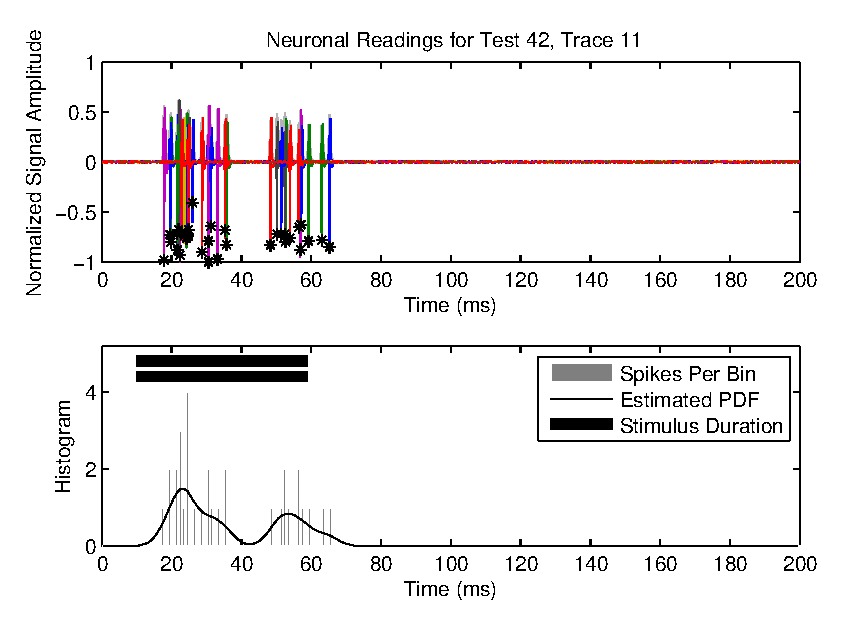
\includegraphics{BasicPlot}\\
  \caption{A typical plot using all of the plotting options}\label{BasicPlot}
\end{center}
\end{figure}


\begin{figure}
\begin{center}
  % Requires \usepackage{graphicx}
  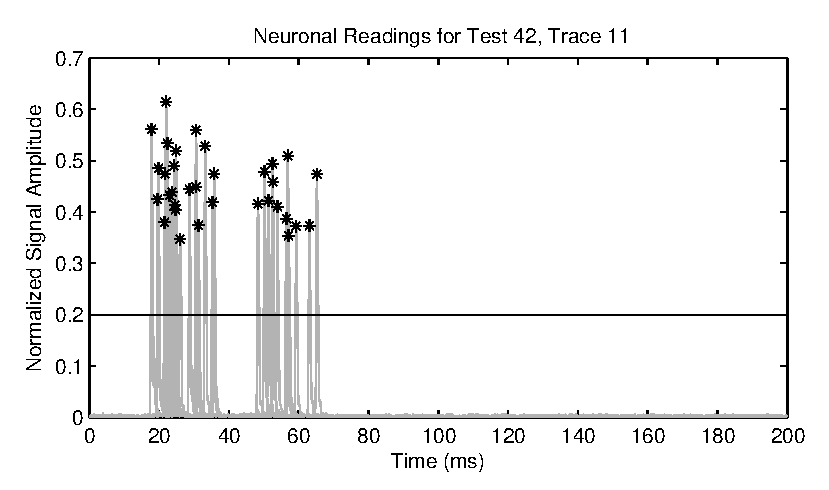
\includegraphics{SpikeDetect}\\
  \caption{A plot showing the power signal used for spike detection and the detected spikes}\label{SpikeDetect}
\end{center}
\end{figure}

\begin{figure}
\begin{center}
  % Requires \usepackage{graphicx}
  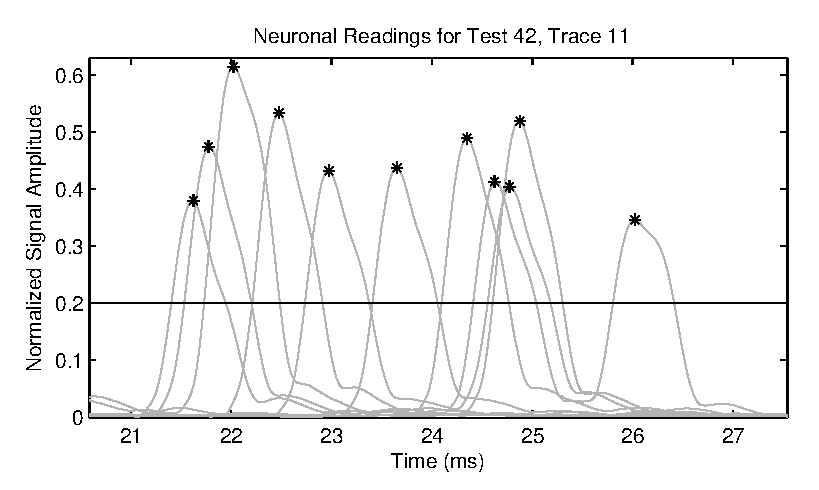
\includegraphics{ZoomSpikeDetect}\\
  \caption{Zoomed in view of Figure \ref{SpikeDetect}}\label{ZoomSpikeDetect}
\end{center}
\end{figure}

\begin{footnotesize}
\begin{alltt}
function PlotData(experiment_data, test_num, trace_num, plot_flag)

   INPUT ARGUMENTS
   experiment_data     bat2matlab structure
   test_num            The number of the test to display
   trace_num           The trace of test test_num to display
   plot_flag           A binary vector indicating the plotting features to
                       display
                       Default: [1 1 1 1 1 1]
       flag index 1    Plot the raw MER signals
       flag index 2    Plot the smoothed MER power signals (used for spike
                       detection)
       flag index 3    Plot the detected spikes
       flag index 4    Plot the spike histogram
       flag index 5    Plot the estimated spike histogram PDF (normalized
                       to the integrated histogram for viewing purposes)
       flag index 6    Plot the stimulus
\end{alltt}
\end{footnotesize}
By default, all of the viewing options are "on" (\verb"plot_flag ="
\verb"[1 1 1 1 1 1]"). A typical output is shown in Figure
\ref{BasicPlot}.

The top plot shows the MERs. Each sweep of the trace is shown in a
different color. The asterisks indicate the spikes that were
calculated. They appear at the points of maximum signal power, and
hence don't necessarily occur at the minima or maxima of the spike.
The power of the signals are indicated in grey (they are difficult
to see with the MER signals overlaid).

The bottom plot of Figure \ref{BasicPlot} shows the histogram of the
detected spikes in grey. The horizontal black lines indicate the
duration of the stimulus in the test. In this case, the test
consisted of two tones being presented. Each starts at 10
milliseconds and is 50 milliseconds in duration

By turning off the plotting of the spikes and the histogram features
(e.g., by setting \verb"plot_flag" to \verb"[0 1 1 0 0 0]"), one can
view the power of the MER signals, the power peaks used for spike
detection, and the threshold used for the detection. The same data
used in Figure \ref{BasicPlot} viewed in this format is shown in
Figure \ref{SpikeDetect}. Figure \ref{ZoomSpikeDetect} shows a
zoomed in view of Figure \ref{SpikeDetect}. Here, it is clear that
the peaks of the MER power are well above the default threshold and
the noise floor is well below.


\section{Example}
The following example assumes that the Batlab XML file has already
been generated from the PST file using the Batgor program. Both the
XML and raw data files are needed to use Bat2Matlab. Running the
example will generate the plots in Figures \ref{BasicPlot} and
\ref{SpikeDetect}.

\begin{footnotesize}
\begin{alltt}
raw_data_filepath = 'bat 7b.raw';
xml_data_filepath = 'bat 7b-alltests.xml';
%Extract XML metadata and convert to to Matlab structure
experiment_data = BatlabXml2MatlabStructure(xml_data_filepath);

%Specify which tests to extract raw data from
%This can be in the form [42 46] or [42:52] to specify multiple tests
test_nums_to_extract = 42;

experiment_data = ExtractRawData(experiment_data,raw_data_filepath,test_nums_to_extract);
experiment_data = CalculateSpikeTimes(experiment_data,test_nums_to_extract);
experiment_data = GenerateHistograms(experiment_data,test_nums_to_extract);

%Specify the trace number to view
trace_num = 11;
PlotData(experiment_data,test_nums_to_extract,trace_num,[1 1 1 1 1 1]);
PlotData(experiment_data,test_nums_to_extract,trace_num,[0 1 1 0 0 0]);
\end{alltt}
\end{footnotesize}


\section{Appendix A: Batlab Metadata XML Schema}
\begin{footnotesize}
\begin{alltt}
<?xml version="1.0" encoding="UTF-8" ?>\\
<xs:schema xmlns:xs="http://www.w3.org/2001/XMLSchema">
  <xs:element name="experiment">
    <xs:complexType>
      <xs:sequence>
        <xs:element ref="test" maxOccurs="unbounded" />
      </xs:sequence>
      <xs:attribute name="computername" type="xs:string" use="required" />
      <xs:attribute name="date" type="xs:string" use="required" />
      <xs:attribute name="who" type="xs:string" use="required" />
      <xs:attribute name="pst_filename" type="xs:string" use="required" />
      <xs:attribute name="program_date" type="xs:string" use="required" />
      <xs:attribute name="title" type="xs:string" use="required" />
    </xs:complexType>
  </xs:element>

  <xs:element name="spikedata">
    <xs:complexType mixed="true">
      <xs:attribute name="units" type="xs:string" use="required" />
    </xs:complexType>
  </xs:element>

  <xs:element name="stimulus">
    <xs:complexType>
      <xs:attribute name="soundtype" type="xs:NMTOKEN" use="required" />
      <xs:attribute name="AMdepth" type="xs:decimal" use="optional" />
      <xs:attribute name="AMdutycycle" type="xs:decimal" use="optional"/>
      <xs:attribute name="duration" type="xs:decimal" use="optional" />
      <xs:attribute name="delay" type="xs:decimal" use="optional" />
      <xs:attribute name="reverse_vocal_call" type="xs:NMTOKEN" use="optional" />
      <xs:attribute name="attenuation" type="xs:decimal" use="optional" />
      <xs:attribute name="frequency" type="xs:decimal" use="optional" />
      <xs:attribute name="AMrate" type="xs:decimal" use="required" />
      <xs:attribute name="vocal_call_file" type="xs:NMTOKEN" use="optional" />
      <xs:attribute name="AMtype" type="xs:NMTOKEN" use="required" />
      <xs:attribute name="phase" type="xs:decimal" use="optional" />
      <xs:attribute name="soundtype_name" type="xs:string" use="required" />
      <xs:attribute name="rise_fall" type="xs:NMTOKEN" use="optional" />
    </xs:complexType>
  </xs:element>

  <xs:element name="test">
    <xs:complexType>
      <xs:sequence>
        <xs:element ref="trace" maxOccurs="unbounded" />
      </xs:sequence>
      <xs:attribute name="length_in_raw_file" type="xs:positiveInteger" use="required" />
      <xs:attribute name="date" type="xs:string" use="required" />
      <xs:attribute name="testtype" type="ts:NMTOKEN" use="required" />
      <xs:attribute name="id" type="xs:NMTOKEN" use="required" />
      <xs:attribute name="comment" type="xs:string" use="required" />
    </xs:complexType>
  </xs:element>

  <xs:element name="trace">
    <xs:complexType>
      <xs:all>
        <xs:element ref="spikedata" />
        <xs:element ref="stimulus" />
      </xs:all>
      <xs:attribute name="window_detector_status" type="xs:NMTOKEN" use="required" />
      <xs:attribute name="level_detector_status" type="xs:NMTOKEN" use="required" />
      <xs:attribute name="run_number" type="xs:positiveInteger" use="required" />
      <xs:attribute name="level_voltage" type="xs:decimal" use="required" />
      <xs:attribute name="spike_enhancer_status" type="xs:NMTOKEN" use="required" />
      <xs:attribute name="record_duration" type="xs:positiveInteger" use="required" />
      <xs:attribute name="soundtype" type="xs:NMTOKEN" use="required" />
      <xs:attribute name="window_voltage" type="xs:decimal" use="required" />
      <xs:attribute name="is_control" type="xs:NMTOKEN" use="required" />
      <xs:attribute name="spike_enhancer_power_value" type="xs:decimal" use="required" />
      <xs:attribute name="length_in_raw_file" type="xs:positiveInteger" use="required" />
      <xs:attribute name="samplerate_ad" type="xs:positiveInteger" use="required" />
      <xs:attribute name="display_duration" type="xs:decimal" use="required" />
      <xs:attribute name="binwidth" type="xs:positiveInteger" use="required" />
      <xs:attribute name="peak_detector_status" type="xs:NMTOKEN" use="required" />
      <xs:attribute name="samplerate_da" type="xs:positiveInteger" use="required" />
      <xs:attribute name="invert_raw_data_status" type="xs:NMTOKEN" use="required" />
      <xs:attribute name="num_samples" type="xs:positiveInteger" use="required" />
      <xs:attribute name="repetition_rate" type="xs:positiveInteger" use="required" />
      <xs:attribute name="samplerate_type" type="xs:NMTOKEN" use="required" />
      <xs:attribute name="stats_start" type="xs:positiveInteger" use="required" />
      <xs:attribute name="stats_end" type="xs:positiveInteger" use="required" />
    </xs:complexType>
  </xs:element>
</xs:schema>
\end{alltt}
\end{footnotesize}

\section{Appendix B: Bat2Matlab Structure}
\begin{footnotesize}
\begin{alltt}
experiment.computername
           date
           program_date
           pst_filename
           title
           who
           test.comment
                date
                id
                length_in_raw_file
                offset_in_raw_file
                testtype
                trace.display_duration
                      invert_raw_data_status
                      is_control
                      length_in_raw_file
                      level_detector_status
                      level_voltage
                      num_samples
                      peak_detector_status
                      record_duration
                      repetition_rate
                      run_number
                      samplerate_ad
                      samplerate_da
                      samplerate_type
                      soundtype
                      spike_enhancer_power_value
                      spike_enhancer_status
                      stats_end
                      stats_start
                      window_detector_status
                      window_voltage
                      stimulus
                      raw_data
                      spike_idx
                      spike_times
                      smoothed_data
                      peak_threshold
                      histogram
                      histogram_bin_width
                      histogram_bin_centers
\end{alltt}
\end{footnotesize}



\end{document}
